\subsubsection{ARIB STD-T109}
% 
% Section about Japanese technology ARIB.
\acrshort{arib} STD-T109 is a standard developed by Association of Radio Industries and Businesses, a Japan-based organisation. The standard was developed to \textquote[\cite{2012ARIB1.0}]{\textit{Enable effective use of radio frequencies by avoiding interference among users}}, for use in intelligent transportation systems.\par
% 
The radio communication requirements for \acrfull{arib} consist of single channel radio communication in the 700 MHz band with both \acrshort{V2I} and \acrshort{V2V} communication. The communication have to support \acrshort{V2V} communication up to vehicle speed of 140 km/h and V2I up to vehicle speed of 70 km/h.\par
% 
The protocol stack of ARIB STD-t109 is of a 4 layer-structure.
Layer 1: Physical layer. It consist of 2 sub-layers, \acrfull{PMD} sublayer and \acrfull{PLCP} sublayer. The \acrshort{PMD} sublayer gives a method to transmit and receive data between stations (\acrshort{V2I} or \acrshort{V2V}) that uses \acrshort{OFDM}.
Layer 2: Data link layer. It consist of 2 sublayers, \acrshort{MAC} sublayer and \acrshort{LLC} sublayer. In the \acrshort{MAC} sublayer \acrshort{CSMA} is used for multiple access control method. The \acrshort{LLC} sublayer lets unacknowledged services (data without error control and no guarantee of delivery) to transmit packets between upper layers.
\acrshort{V2V}\&\acrshort{V2I} layer: Inter-vehicle and Roadside-to-vehicle communication layer. It creates and manages data required for \acrshort{V2I} and \acrshort{V2V} communication control. It also makes a method to give parameters needed for communication control for the \acrshort{MAC} sublayer (synchronises clocks etc).
Layer 7: Application layer. It gives a communication control method and services for applications such as security and it also gives a method to transmit and receive data through the V2V\&V2I layer. 
\par
The \acrfull{PDU} of the \acrshort{MAC} and \acrshort{LLC} sublayer can be seen on Figure \ref{fig:PSDU}.
\begin{figure}
    \centering
    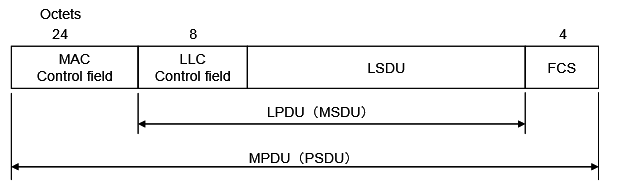
\includegraphics[width=14cm]{PSDU}
    \caption{Shows \acrshort{MAC} protocol in parts}
    \label{fig:PSDU}
\end{figure}

A \acrshort{PDU} of \acrshort{MAC}, called \acrfull{MPDU}, consists of 4 elements. \acrshort{MAC} Control field, \acrshort{LLC} control field, \acrfull{LSDU} and \acrfull{FCS}.
\acrshort{MAC} control field's length is 24 octet and contain information needed to control and establishing connection, it can be broken down to 6 fields with each of their length shown below.
\begin{figure}
    \centering
    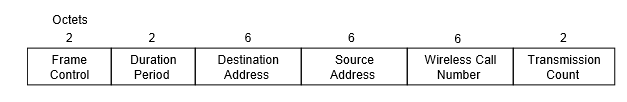
\includegraphics[width=14cm]{MAC}
    \caption{Shows breakdown of \acrshort{MAC} Control field}
    \label{fig:MAC}
\end{figure}

Frame control has the data for what type of frames and fields is coming up. Duration period contains duration value for each frame. Destination Address is the receiver's \acrshort{MAC} address. Source Address is the senders MAC address. Wireless call number is a identification code for security reasons. Transmission count is a number which goes up by 1 for each transmission. 

\acrshort{LLC} control field can be split into 4 fields. \acrfull{DSAP} address field identifies which \acrshort{SAP}s is intended for the \acrshort{LLC} \acrshort{PDU}. \acrfull{SSAP} Address field identifies if the \acrshort{LLC} \acrshort{PDU} is a command or response \acrshort{PDU}. Control field contains command, response, and sequence number information. Protocol identifier field sees if the right protocol is being used.
\begin{figure}[h]
    \centering
    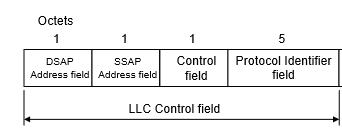
\includegraphics[width=14cm]{LLC-control-field}
    \caption{Shows breakdown of \acrshort{LLC} control field}
    \label{fig:LLC}
\end{figure}
Lastly is the \acrshort{LSDU} and \acrshort{FCS}, which help detect data errors that might have happened during the transmission, by checking if the number based on the data matches the \acrshort{FCS} number, after receiving the data. 
\par
% 
Though \acrshort{arib} T109 is using the same physical layer as \acrshort{IEEE} 802.11, one of the key differences is that the \acrshort{MAC} address not only is being used to identify which \acrshort{SAP}s of the layers but also to distinguish between communication traffic between \acrshort{V2V} and \acrshort{V2I}. The \acrshort{TDMA} (Time-division multiple access) scheme is used by having control cycles of 100.000$\upmu$s which is then divided into 16 smaller cycles of  6240$\upmu$s. Each of the small cycles have 2 periods, the first period, 0 to 3024$\upmu$s is called V2I period which is the period where only that form of communication access is allowed in the channel. The reason is that the infrastructure is connected to multiple sensors scattered around the road, giving it more knowledge about the current situation than a vehicle for distributing safety information. Since each infrastructure can be allocated a specific time-slot in the V2I period, it is not necessary to use \acrshort{CSMA}. After the \acrshort{V2I} period ends (after 3024$\upmu$s), vehicles can compete for channel access, but to avoid concurrent channel access with other vehicles, \acrshort{CSMA} is used \cite{Heinovski2016PerformanceSTD-T109}.\par
% 
Like the \acrshort{IEEE} 802.11 and \acrshort{ETSI}, \acrshort{arib} also uses \acrshort{OFDM} for multiplexing. \acrshort{OFDM} uses \acrshort{BPSK}, \acrshort{QPSK}, 16-QAM and 64-QAM as modulation schemes\footnotemark.\par
% 
\footnotetext{\url{http://rfmw.em.keysight.com/wireless/helpfiles/n7617a/coding_and_modulation.htm}, accessed on 17/04/2017}
% 
\acrshort{arib} T109, using both \acrshort{TDMA} and \acrshort{CSMA} (compare to 802.11p only using \acrshort{CSMA}) gives it a better communication distance in urban environment almost up to 3 times the distance \cite{Heinovski2016PerformanceSTD-T109}, because it suffers less from obstacles such as buildings etc. On the other hand, because of the priority of the \acrshort{V2I} period, it causes packet losses for the traffic between vehicles. For same reason, message delays also happen, since they need to wait for the next time slot, which is not reserved, and this causes delay. 